\documentclass[11pt]{article}
\usepackage[norsk]{babel}
\usepackage[utf8]{inputenc}
\usepackage{alltt}
\usepackage{listings}
\usepackage{hyperref}
\usepackage{color}
\usepackage{amsmath}
\usepackage{amssymb}
\usepackage{amsthm}
\usepackage{wasysym}
\usepackage{lipsum}
\usepackage{sectsty}
\usepackage{fullpage}
\usepackage{graphicx}
\usepackage{import}
\usepackage{cancel}
\usepackage{pdfpages}
\usepackage{siunitx}
        \DeclareSIUnit\gauss{G}
	\sisetup{exponent-product = \cdot}	% Prikk som multiplikasjonstegn (i stedet for kryss).
 	\sisetup{output-decimal-marker  =  {.}}	% Punktum som desimalskilletegn (i stedet for komma).
 	\sisetup{separate-uncertainty = true} 	% Pluss-minus-form på
                                % usikkerhet (i stedet for parentes). 
\usepackage{pgfplots}
\pgfplotsset{compat=1.9}
\usepackage{comment}

% Denne setter navnet på abstract til Sammendrag
% \renewenvironment{abstract}{\global\setbox\absbox=\vbox\bgroup
% \hsize=\textwidth\def\baselinestretch{1}%
% \noindent\unskip\textbf{Sammendrag}
% \par\medskip\noindent\unskip\ignorespaces}
% {\egroup}

% Disse kommandoene definerer hvor stor andel av siden som kan være dekket av figurer. Kan gjøre det enklere å plassere figurer.
\setcounter{totalnumber}{15}
\renewcommand{\textfraction}{0.05}
\renewcommand{\topfraction}{0.95}
\renewcommand{\bottomfraction}{0.95}
\renewcommand{\floatpagefraction}{0.35}


%\renewcommand{\theequation}{(\thesubsection.hei\arabic{equation})}
\newcommand\numberthis{\addtocounter{equation}{1}\tag{\theequation}}
\renewcommand{\thesection}{\arabic{section}}
\renewcommand{\thesubsection}{\alph{subsection})}
%\renewcommand{\thesubsection}{\thesection.\alph{subsection})} % subsection is now 1.a), 1.b)... 2.a)...

%\allsectionsfont{\centering \normalfont} % Make all sections centered, the default font

\usepackage{fancyhdr} % Custom headers and footers
\pagestyle{fancyplain} % Makes all pages in the document conform to the custom headers and footers
\fancyhead[C]{\footnotesize \textit{FYS3150 Prosjekt 1\\ $ \,$}} % No page header - if you want one, create it in the same way as the footers below
\fancyhead[R]{} \fancyhead[L]{} \fancyfoot[L]{} % Empty left footer
\fancyfoot[C]{} % Empty center footer
\fancyfoot[R]{\thepage} % Page numbering for right footer
\renewcommand{\headrulewidth}{0pt} % Remove header underlines
\renewcommand{\footrulewidth}{0pt} % Remove footer underlines
\setlength{\headheight}{21pt} % Customize the height of the header

% \numberwithin{equation}{subsection} % Number equations within sections (i.e. 1.1, 1.2, 2.1, 2.2 instead of 1, 2, 3, 4)
% \numberwithin{figure}{section} % Number figures within sections (i.e. 1.1, 1.2, 2.1, 2.2 instead of 1, 2, 3, 4)
% \numberwithin{table}{section} % Number tables within sections (i.e. 1.1, 1.2, 2.1, 2.2 instead of 1, 2, 3, 4)


\definecolor{yellow}{rgb}{0.7,0.8,0}
%\definecolor{blue}{rgb}{0,0,0.8}
\definecolor{blue}{rgb}{0.3,0.3,0.9}
\definecolor{green}{rgb}{0,0.3,0}
\lstloadlanguages{Python} 
\lstloadlanguages{MATLAB}
\lstloadlanguages{C}
\lstset{%frame=single, % Single frame around code
		otherkeywords={self},
        keywordstyle=\color{blue},
        commentstyle=\color{green},
        stringstyle=\color{green}, % Strings are green
        showstringspaces=false, % Don't put marks in string spaces
        tabsize=5, % 5 spaces per tab        
        numbers=none, % Line numbers on left
        %firstnumber=1, % Line numbers start with line 1
        stepnumber=1 % Line numbers go in steps of 5
}


\newcommand{\horline}{
\begin{center}
\line(1,0){350}
\end{center}
}


% common commands
\newcommand{\pd}[2] {\frac{\partial #1}{\partial #2}}
\renewcommand{\div}[1] {\nabla\cdot\vec{#1}}
\newcommand{\curl}[1] {\nabla\times\vec{#1}}
\renewcommand{\vec}{\mathbf} % bold face for vectors
\newcommand{\e}[1] {\times 10^{#1}}
\newcommand{\mean}[1] {\langle #1 \rangle}


\begin{document}
% make title page
\begin{titlepage}
\newcommand{\HRule}{\rule{\linewidth}{0.5mm}}
\center
\textsc{\LARGE Universitetet i Oslo}\\[1.5cm] % Name of your university/college
\textsc{\Large }\\[0.5cm] % Major heading such as course name
\textsc{\large FYS3150}\\[0.5cm] % Minor heading such as course title
\HRule \\[0.4cm]
{ \huge \bfseries Prosjekt 1 }\\[0.4cm] % Title of your document
\HRule \\[1.5cm]
\Large \emph{Skrevet av:}\\
Lyder \textsc{Rumohr Blingsmo} og Bendik \textsc{Samseth}\\[3cm]
{\large \today}\\[3cm]
\vfill
\end{titlepage}


\begin{abstract}
I dette prosjektet skal vi kjent med ulike vektor- og
matriseoperasjoner. Vi skal benytte C++ for størsteparten av
beregningene i et forsøk på å bli bedre kjent med språket. Vi ser på
andreordens lineære differensialligninger, spesielt ser vi på den
generelle endimensjonelle Poisson ligningen med Dirichlet
randbetingelser. Vi ser på flere måter å løse slike systemer, og
analyserer forskjellene med tanke på kjøretid og nøyaktighet.
\end{abstract}


Vi har gitt den generelle formen til den endimensjonelle
Possionsligningen:
\begin{align}
  -u''(x) = f(x)\label{eq:poisson}
\end{align}
med $x \in (0,1)$ og $u(0) = u(1) = 0$.

\subsection{}

For å komme frem til en numerisk løsning til \eqref{eq:poisson}
definerer vi den diskretiserte tilnærmingen til $u(x)$ som $v_i$ med
x-verdier $x_i = ih$ på intervallet $x_0 = 0$ og $x_{n+1} =
1$. Avstanden mellom hver $x_i$ defineres som $h =
1/(n+1)$. Randbetingelsene blir da $v_0 = v_{n+1} = 0$.

Ligning \eqref{eq:poisson} viser at vi trenger den dobbeltderiverte av
$u(x)$. For $v_i$ kan vi tilnærme dette som 

\begin{align}
  - \frac{ v_{i+1} + v_{i-1} - 2v_i }{ h^2 } =
  f_i\hspace{1cm}\text{for } i = 1,\dots,n.
\end{align}
der $f_i = f(x_i)$. Vi setter 
\begin{align*}
      {\bf A} = \left(\begin{array}{cccccc}
                           2& -1& 0 &\dots   & \dots &0 \\
                           -1 & 2 & -1 &0 &\dots &\dots \\
                           0&-1 &2 & -1 & 0 & \dots \\
                           & \dots   & \dots &\dots   &\dots & \dots \\
                           0&\dots   &  &-1 &2& -1 \\
                           0&\dots    &  & 0  &-1 & 2 \\
                      \end{array} \right)
\end{align*}
Da ser vi at $\vec A \vec v$ blir lik 
\begin{align*}
  \vec A \vec v = -v_{i+1} - v_{i-1} + 2v_i\hspace{1cm}\text{for } i = 1,\dots,n
\end{align*}
når vi har at $v_0 = v_{n+1} = 0$ fra Dirichlet-randbetingelsene. Hvis
vi definerer $\vec d$ ved $d_i = h^2f_i$ kan vi skrive
\eqref{eq:poisson} som 
\begin{align}
  \vec A \vec v = \vec d.\label{Av=d}
\end{align}
 

Vi skal videre anta at $f(x) = 100 e^{-10x}$. Da har
\eqref{eq:poisson} en eksakt løsning gitt som
 \begin{align}
u(x) = 1 -\left(1-e^{-10}\right) - e^{-10x}.\label{eq:exact}
\end{align} 
Vi skal bruke denne til å
sammenlikne med vår numeriske lønning i senere oppgaver.

\subsection{}
For å løse \eqref{Av=d} skal vi benytte en noen modifisert version av
Thomas algoritmen\footnote{Se
  \url{https://en.wikipedia.org/wiki/Tridiagonal_matrix_algorithm}}. Denne
algoritmen kan beskrives som følger: 

Gitt 
\begin{align*}
  \begin{bmatrix}
   {b_1} & {c_1} &  &  & \text{\huge0} \\
   {a_2} & {b_2} & {c_2} &  &  \\
    & {a_3} & {b_3} & \ddots &  \\
    &  & \ddots & \ddots & {c_{n-1}}\\
     \text{\huge0}&  &  & {a_n} & {b_n}\\
\end{bmatrix}
\begin{bmatrix}
   {x_1 }  \\
   {x_2 }  \\
   {x_3 }  \\
   \vdots   \\
   {x_n }  \\
\end{bmatrix}
=
\begin{bmatrix}
   {d_1 }  \\
   {d_2 }  \\
   {d_3 }  \\
   \vdots   \\
   {d_n }  \\
\end{bmatrix}.
\end{align*}
Vi kan løse systemet ved å utføre en forward-substitution bestående av
å bytte ut matrise elementene med $c_i'$ og $d_i'$ på følgende måte.
\begin{align*}
  c_i' &= \begin{cases}
\begin{array}{lcl}
  \cfrac{c_i}{b_i}                  & ; & i = 1 \\
  \cfrac{c_i}{b_i - a_i c'_{i - 1}} & ; & i = 2, 3, \dots, n-1 \\
\end{array}
\end{cases}\\
d_i' &= \begin{cases}
\begin{array}{lcl}
  \cfrac{d_i}{b_i}                  & ; & i = 1 \\
  \cfrac{d_i - a_i d'_{i - 1}}{b_i - a_i c'_{i - 1}} & ; & i = 2, 3, \dots, n. \\
\end{array}
\end{cases}
\end{align*}
Deretter finner vi løsningen ved backward-substitution.
\begin{align*}
  x_n &= d'_n\\
  x_i &= d'_i - c'_i x_{i + 1} \qquad ; \ i = n - 1, n - 2, \ldots, 1.
\end{align*}

Dette teller vi til å tilsvare $\mathcal{O}(10n)$ FLOPS. Siden vi i
vårt tilfellet har like elementer på diagonalene, kan vi trimme dette
ned litt. 

Siden $a_i = -1\ \forall\  i$ og  $b_i - a_ic_{i-1}'$ er felles nevner
for både $c_i'$ og $d_i'$ kan vi gjøre om forward-substitution til det følgende:

\begin{align*}
  c_i' &= \begin{cases}
\begin{array}{lcl}
  \cfrac{c}{b}                  & ; & i = 1 \\
  \cfrac{c}{b + c'_{i - 1}} & ; & i = 2, 3, \dots, n-1 \\
\end{array}
\end{cases}\\
d_i' &= \begin{cases}
\begin{array}{lcl}
  \cfrac{d_i}{b}                  & ; & i = 1 \\
  \cfrac{d_i + d'_{i - 1}}{b + c'_{i - 1}} & ; & i = 2, 3, \dots, n. \\
\end{array}
\end{cases}
\end{align*}
Her kan vi spare operasjoner ved å bare beregne $b+c'_{i-1}$ en gang
(for alle $i$) og bruke resultatet både for beregningen av $c_{i}'$ og
$d_{i}'$.

Med disse endringene teller vi antall operasjoner til å gå som
$\mathcal{O}(6n)$. Dette er en betydelig raskere algoritme sammenliket
med standard Gauss eliminasjon. I følge forelesningsnotatene går
vanlig Gauss eliminasjon som $\mathcal{O}(\frac{ 2 }{ 3 }n^3)$. I
tillegg krever ikke algoritmen vi bruker at vi lagrer en full
matrise. Tridiagonale matriser med stor $n$ inneholder veldig mange
nuller, så det er smart å ikke trenge å lagre all den unødvendige
informasjonen. Dette gjør oss i stand til å løse matriser av mye
større dimensjon sammenliknet med når vi er nødt til å lagre den fulle matrisen.

Vi har implementert dette i C++ slik\footnote{Hele programfilen er å
  finne på Github-siden \url{https://github.com/bsamseth/fys3150-project1.git}}:
\begin{lstlisting}[language=C]
void tridiagonal( double b, double c, double * d, double * v ) {
    /* Function for solving the eq. Av=d in the case 
       that A is tridiagonal, with a constant value on the diagonals.
       Specialy the subdiagonal must be equal to -1.

       b - value for the main diagonal
       c - value for the superdiagonal
       d - a vector with the function values
       v - souluiton vector. Will be filled when function returns
       N - dimension of the matrix/vectors

       Using the Thomas Algorithm, with modifications.
    */
    int i;
    double * c_prime = new double[N];

    /* The loop below will depend on c_prime[i-1] and 
       d[i-1] to be already changed, so c_prime[0] and 
       d[0] will be set manually at first */
    
    c_prime[0] = c / b;
    d[0] = d[0] / b;

    double m;
    for (i = 1; i < N; i++) {
	m = 1.0 / (b + c_prime[i-1]);
	c_prime[i] = c * m;
	d[i] = (d[i] + d[i-1]) * m;
    }

    v[N-1] = d[N-1];
    for (i = N - 1; i-- > 0; ) {
	v[i] = d[i] - c_prime[i] * v[i+1];
    }
}
\end{lstlisting}

Figur \ref{fig:b} viser resultatet av å bruke denne algoritmen med
$N = \{10,100,1000\}$. Vi ser at $v_i$ konvergerer raskt mot $u(x)$
når vi øker verdien av N. For $N=1000$, (som forøvrig ikke virker å ta
merkbart mer tid å lage sammenliket med lavere N) er det vanskelig å
skille den eksakte fra tilnærmingen. Det virker med dette som
algoritmen vi har skrevet fungerer som ønsket.

\begin{figure}[ht]
  \centering
  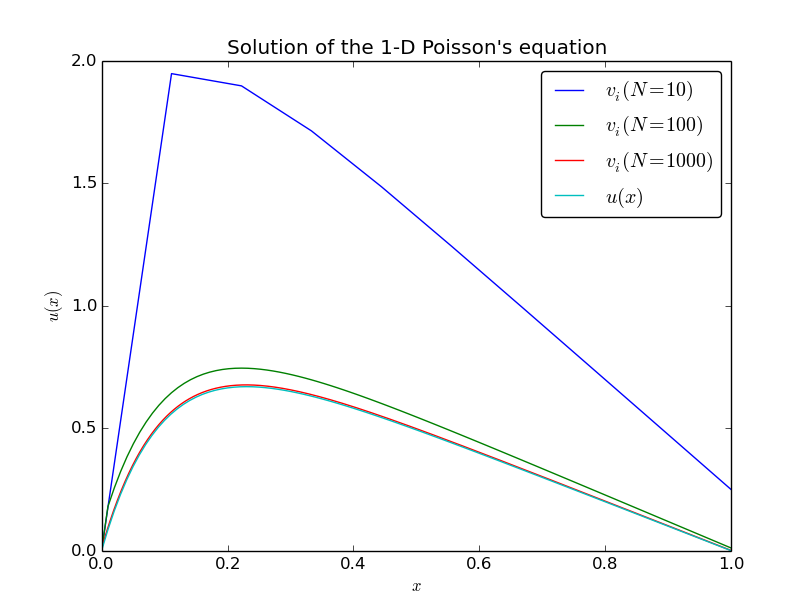
\includegraphics[scale=0.7]{fig/b.png}
  \caption{\label{fig:b} Løsninger av \eqref{eq:poisson} for
    forskjelige verider av N. $u(x)$ viser kurven til den eksakte løsningen.}
\end{figure}



\end{document}
%%% Local Variables: 
%%% mode: latex
%%% TeX-master: t
%%% End: 


















